 
\chapter{Transformations in OLS}
 
Transforming the outcome and covariates is fundamental in linear models. Whenever we specify a linear model $y_i = x_i^{\T} \beta + \varepsilon_i$, we implicitly have transformed the original $y$ and $x$, or at least we have chosen the scales of them. 
\citet{carroll1988transformation} is a textbook on this topic. 
This chapter discusses some important special cases. 


\section{Transformation of the outcome}

Although we can view
\[
y_{i}=x_{i}^{\T}\beta+\varepsilon_{i},\quad(i=1,\ldots,n)
\]
as a linear projection that works for any type of outcome $y_{i}\in\mathbb{R}$,
the linear model works the best for continuous outcomes and especially
for Normally distributed outcomes. Sometimes, the linear model can be a poor approximation of the original outcome but may perform well for certain transformations of the outcome. 

\subsection{Log transformation}

With positive, especially heavy-tailed outcomes, a standard transformation
is the log transformation. So we fit a linear model
\[
\log y_{i}=x_{i}^{\T}\beta+\varepsilon_{i},\quad(i=1,\ldots,n).
\]
The interpretation of the coefficients changes a little bit. Because
\[
\frac{\text{\ensuremath{\partial\log}}\hat{y}_{i}}{\partial x_{ij}}=\frac{\partial\hat{y}_{i}}{\hat{y}_{i}}\Big/\partial x_{ij}=\hat{\beta}_{j},
\]
we can interpret $\hat{\beta}_{j}$ in the following way: ceteris
paribus, if $x_{ij}$ increases by one unit, then the proportional
increase in the average outcome is $\hat{\beta}_{j}$. In economics, $\hat{\beta}_{j}$ is the {\it semi-elasticity} of $y$ on $x_j$ in the model with log transformation on the outcome. 


Sometimes, we may apply the log transformation on both the outcome and a certain covariate:
$$
\log y_i = \beta_1 x_{i1}  +\cdots + \beta_j \log x_{ij} + \cdots + \varepsilon_i,\quad(i=1,\ldots,n).
$$
The $j$th fitted coefficient becomes
$$
\frac{\text{\ensuremath{\partial\log}}\hat{y}_{i}}{\partial \log x_{ij}} 
= \frac{\partial\hat{y}_{i}}{\hat{y}_{i}}\Big/ \frac{\partial x_{ij}}{x_{ij}}=\hat{\beta}_{j},
$$
so ceteris
paribus, if $x_{ij}$ increases by $1\%$, then   the average outcome will increase by $\hat{\beta}_{j} \%$. In economics, $\hat{\beta}_{j}$ is the {\it $x_j$-elasticity} of $y$ in the model with log transformation on both the outcome and $x_{j}$. 


The log transformation only works for positive variables. 
For a nonnegative outcome, we can modify the log transformation to $\log (y_{i} + 1).$ 



\subsection{Box--Cox transformation}

Power transformation is another important class.
The Box--Cox transformation unifies the log transformation and the
power transformation:
\[
g_{\lambda}(y)=\begin{cases}
\frac{y^{\lambda}-1}{\lambda}, & \lambda\neq0,\\
\log y, & \lambda=0.
\end{cases}
\]
L'H\^opital's rule implies that 
\[
\lim_{\lambda\rightarrow0}\frac{y^{\lambda}-1}{\lambda}=\lim_{\lambda\rightarrow0}\frac{\d y^{\lambda}/\d\lambda}{1}=\lim_{\lambda\rightarrow0}y^{\lambda}\log y=\log y,
\]
so as a function of $\lambda$, $g_{\lambda}(y)$ is continuous at
$\lambda = 0$. The log transformation is a limiting version of the power transformation. Can we choose $\lambda$ based on data? \citet{box1964analysis} proposed
a strategy based on the maximum likelihood under the Normal linear model:
\[
Y_{\lambda}=\left(\begin{array}{c}
y_{\lambda1}\\
\vdots\\
y_{\lambda n}
\end{array}\right)=\left(\begin{array}{c}
g_{\lambda}(y_{1})\\
\vdots\\
g_{\lambda}(y_{1})
\end{array}\right)\sim\N(X\beta,\sigma^{2}I_{n}).
\]
The density function of $Y_{\lambda}$ is 
\[
f(Y_{\lambda})=(2\pi\sigma^{2})^{-n/2}\exp\left\{ -\frac{1}{2\sigma^{2}}(Y_{\lambda}-X\beta)^{\T}(Y_{\lambda}-X\beta)\right\} .
\]
The Jacobian of the transformation from $Y$ to $Y_{\lambda}$ is
\[
\det\left(\frac{\partial Y_{\lambda}}{\partial Y}\right)=\det\left(\begin{array}{cccc}
y_{1}^{\lambda-1}\\
 & y_{2}^{\lambda-1}\\
 &  & \ddots\\
 &  &  & y_{n}^{\lambda-1}
\end{array}\right)=\prod_{i=1}^{n}y_{i}^{\lambda-1},
\]
so the density function of $Y$ is 
\[
f(Y)=(2\pi\sigma^{2})^{-n/2}\exp\left\{ -\frac{1}{2\sigma^{2}}(Y_{\lambda}-X\beta)^{\T}(Y_{\lambda}-X\beta)\right\} \prod_{i=1}^{n}y_{i}^{\lambda-1}.
\]
If we treat the density function of $Y$ as a function of $(\beta,\sigma^{2},\lambda)$,
then it is the likelihood function, defined as $L(\beta,\sigma^{2},\lambda).$
Given $(\sigma^{2},\lambda)$, maximizing the likelihood function
is equivalent to minimizing $(Y_{\lambda}-X\beta)^{\T}(Y_{\lambda}-X\beta)$,
i.e., we can run OLS of $Y_{\lambda}$ on $X$ to obtain 
\[
\hat{\beta}(\lambda)=(X^{\T}X)^{-1}X^{\T}Y_{\lambda}.
\]
Given $\lambda$, maximizing the likelihood function is equivalent
to first obtaining $\hat{\beta}(\lambda)$ and then obtaining $\hat{\sigma}^{2}(\lambda)=n^{-1}Y_{\lambda}(I_{n}-H)Y_{\lambda}.$
The final step is to maximize the profile likelihood as a function
of $\lambda$:
\[
L(\hat{\beta}(\lambda),\hat{\sigma}^{2}(\lambda),\lambda)=\left\{ 2\pi\hat{\sigma}^{2}(\lambda)\right\} ^{-n/2}\exp\left\{ -\frac{n\hat{\sigma}^{2}(\lambda)}{2\hat{\sigma}^{2}(\lambda)}\right\} \prod_{i=1}^{n}y_{i}^{\lambda-1}.
\]
Dropping some constants, the log profile likelihood function of $\lambda$
is
\[
l_{\textsc{p}}(\lambda)=-\frac{n}{2}\log\hat{\sigma}^{2}(\lambda)+(\lambda-1)\sumn\log y_{i}.
\]


The \ri{boxcox} function in the  \ri{R} package \ri{MASS} plots $l_{\textsc{p}}(\lambda)$, finds it
maximizer $\hat{\lambda}$, and construct a 95\% confidence
interval $[\hat{\lambda}_{\textsc{l}},\hat{\lambda}_{\textsc{U}}]$
based on the following asymptotic pivotal quantity
\[
2\left\{ l_{\textsc{p}}(\hat{\lambda})-l_{\textsc{p}}(\lambda)\right\} \asim\chi_{1}^{2},
\]
which holds by Wilks' Theorem. In practice, we often use the $\lambda$
values within $[\hat{\lambda}_{\textsc{l}},\hat{\lambda}_{\textsc{U}}]$
that have more scientific meanings.


I use two datasets to illustrate the Box--Cox transformation, with the \ri{R} code in \ri{code16.1.2.R}. For the \ri{jobs} data, $\lambda = 2$ seems a plausible value. 
\begin{lstlisting}
library(MASS)
library(mediation)
par(mfrow = c(1, 3))
jobslm = lm(job_seek ~ treat + econ_hard + depress1 + sex + age + occp + marital + 
              nonwhite + educ + income, data = jobs)
boxcox(jobslm, lambda = seq(1.5, 3, 0.1), plotit = TRUE)
jobslm2 = lm(I(job_seek^2) ~ treat + econ_hard + depress1 + sex + age + occp + marital + 
               nonwhite + educ + income, data = jobs)
hist(jobslm$residuals, xlab = "residual", ylab = "", 
     main = "job_seek", font.main = 1)
hist(jobslm2$residuals, , xlab = "residual", ylab = "", 
     main = "job_seek^2", font.main = 1)
\end{lstlisting}

\begin{figure}[ht]
\centering
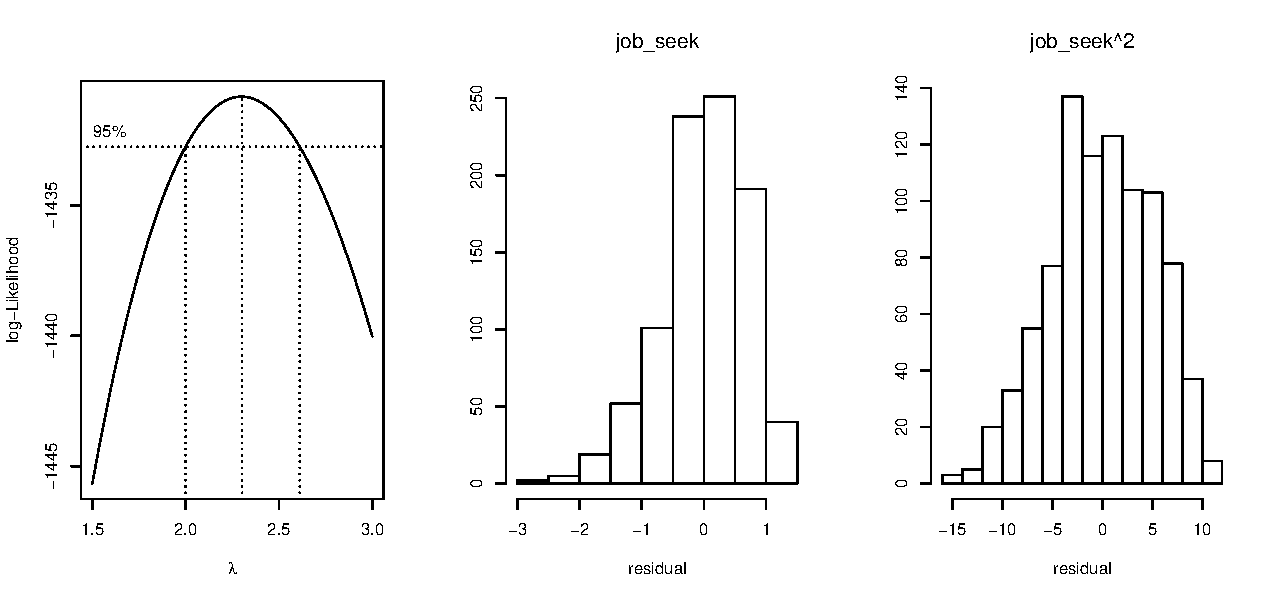
\includegraphics[width = 0.95 \textwidth]{figures/boxcox_jobs.pdf}
\caption{Box--Cox transformation in the \ri{jobs} data} \label{fig::boxcox-jobs}
\end{figure}

In the Penn bonus experiment data, $\lambda = 0.3$ seems a plausible value. However, the residual plot does not seem Normal, making the Box--Cox transformation not very meaningful.  

\begin{lstlisting}
penndata = read.table("pennbonus.txt")
par(mfrow = c(1, 3))
pennlm = lm(duration ~ ., data = penndata)
boxcox(pennlm, lambda = seq(0.2, 0.4, 0.05), plotit = TRUE)

pennlm.3 = lm(I(duration^(0.3)) ~., data = penndata)

hist(pennlm$residuals, xlab = "residual", ylab = "", 
     main = "duration", font.main = 1)
hist(pennlm.3$residuals, xlab = "residual", ylab = "", 
     main = "duration^0.3", font.main = 1)
\end{lstlisting}


\begin{figure}[ht]
\centering
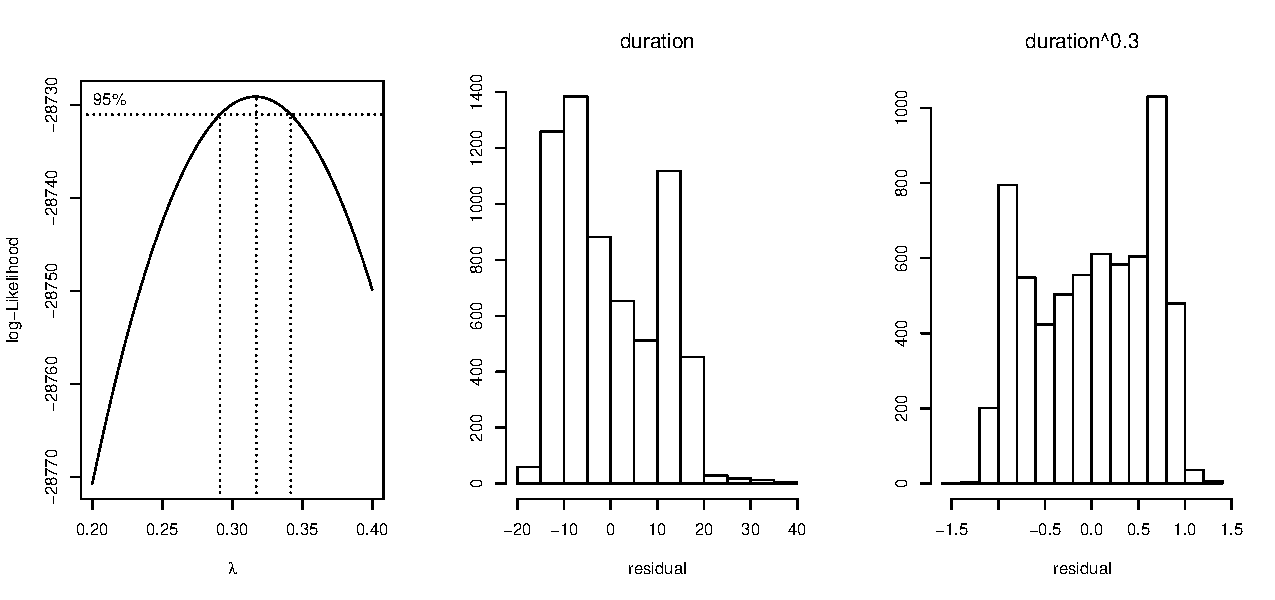
\includegraphics[width =0.95 \textwidth]{figures/boxcox_penn.pdf}
\caption{Box--Cox transformation in the Penn bonus experiment data} \label{fig::boxcox-penn}
\end{figure}

\section{Transformation of the covariates}

%\subsection{Dummy variable}
%
%If a covariate is a factor taking $k$ discrete values, then we can
%create $k-1$ dummy variables indicating $k-1$ levels with the rest
%as the reference level. 
%
% 



\subsection{Polynomial, basis expansion, and generalized additive model}\label{eq::basis-expansion}

Linear approximations may not be adequate, so we can consider a polynomial
specification. With one-dimensional $x$, we can use 
\[
y_{i}=\beta_{1}+\beta_{2}x_{i}+\beta_{3}x_{i}^{2}\cdots+\beta_{p}x_{i}^{p-1}+\varepsilon_{i}.
\]
In economics, it is almost the default choice to include the quadratic term of working experience in the log wage equation. I give an example below using the data from \citet{angrist2006quantile}. The quadratic term of \ri{exper} is significant. 


\begin{lstlisting}
> library(foreign)
> census00 = read.dta("census00.dta")
> head(census00)
  age educ    logwk     perwt exper exper2 black
1  48   12 6.670576 1.0850021    30    900     0
2  42   13 6.783905 0.9666383    23    529     0
3  49   13 6.762383 1.2132297    30    900     0
4  44   13 6.302851 0.4833191    25    625     0
5  45   16 6.043386 0.9666383    23    529     0
6  43   13 5.061138 1.0850021    24    576     0
> 
> census00ols1 = lm(logwk ~ educ + exper + black, 
+                   data = census00)
> census00ols2 = lm(logwk ~ educ + exper + I(exper^2) + black, 
+                   data = census00)
> round(summary(census00ols1)$coef, 4)
            Estimate Std. Error  t value Pr(>|t|)
(Intercept)   4.8918     0.0315 155.0540   0.0000
educ          0.1152     0.0012  99.1472   0.0000
exper         0.0002     0.0008   0.2294   0.8185
black        -0.2466     0.0085 -29.1674   0.0000
> round(summary(census00ols2)$coef, 4)
            Estimate Std. Error  t value Pr(>|t|)
(Intercept)   5.0777     0.0887  57.2254   0.0000
educ          0.1148     0.0012  97.6506   0.0000
exper        -0.0148     0.0067  -2.2013   0.0277
I(exper^2)    0.0003     0.0001   2.2425   0.0249
black        -0.2467     0.0085 -29.1732   0.0000
\end{lstlisting}


We can also include polynomial terms of more than one covariate, for example,
$$
(1,x_{1i},\ldots,x_{i1}^{d},x_{i2},\ldots,x_{i2}^{l})
$$
or 
$$
(1,x_{1i},\ldots,x_{i1}^{d},x_{i2},\ldots,x_{i2}^{l},x_{i1}x_{i2},\ldots,x_{i1}^{d}x_{i2}^{l}).
$$
 


We can also approximate the conditional mean function of the outcome by a linear combination of some basis functions:
\begin{eqnarray*}
y_{i} &=& f(x_{i})+\varepsilon_{i} \\
& \cong & \sum_{j=1}^{J}\beta_{j}S_{j}(x_{i})+\varepsilon_{i},
\end{eqnarray*}
where the $S_{j}(x_{i})$'s are basis functions. The \ri{gam} function in the \ri{mgcv} package uses this strategy including the automatic procedure of choosing the number of basis functions $J$. The following example has a sine function as the truth, and the basis expansion approximation yields reasonable performance with sample size $n=1000$. Figure \ref{fig::npreg-basis} plots both the true and estimated curves.

\begin{lstlisting}
library(mgcv)
n = 1000
dat = data.frame(x <- seq(0, 1, length.out = n),
                 true <- sin(x*10),
                 y <- true + rnorm(n))
np.fit = gam(y ~ s(x), data = dat)
plot(y ~ x, data = dat, bty = "n",
     pch = 19, cex = 0.1, col = "grey")
lines(true ~ x, col = "grey") 
lines(np.fit$fitted.values ~ x, lty = 2)
legend("bottomright", c("true", "estimated"), 
       lty = 1:2, col = c("grey", "black"), 
       bty = "n")
\end{lstlisting} 




\begin{figure}
\centering 
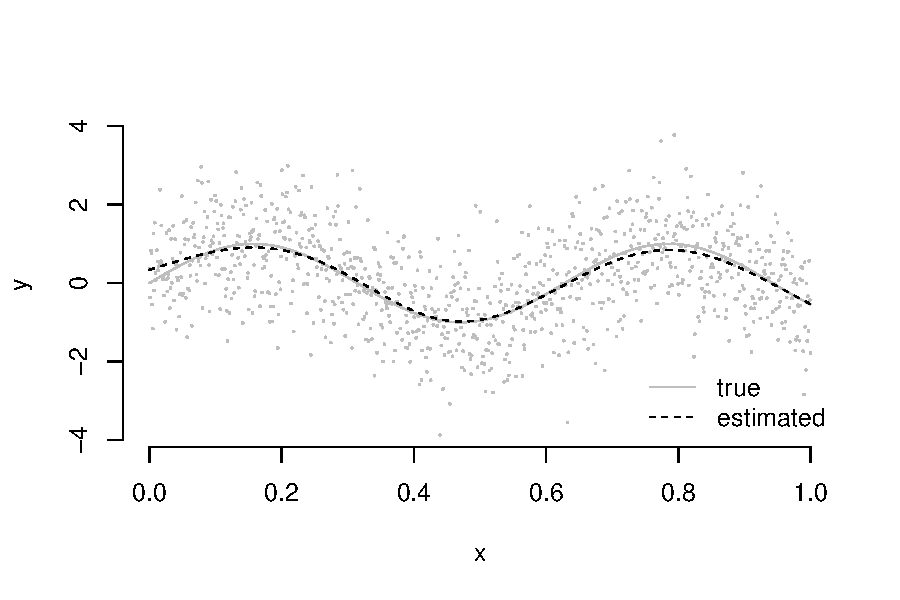
\includegraphics[width =  \textwidth]{figures/npregbasis.pdf}
\caption{Nonparametric regression using the basis expansion}\label{fig::npreg-basis}
\end{figure}


The generalized additive model is an extension of the multivariate case: 
\begin{align*}
y_{i} & =f_{1}(x_{i1})+\cdots+f_{p}(x_{ip})+\varepsilon_{i}\\
 & \cong\sum_{j=1}^{J_{1}}\beta_{1j}S_{j}(x_{i1})+\cdots+\sum_{j=1}^{J_{p}}\beta_{pj}S_{j}(x_{ip})+\varepsilon_{i}.
\end{align*}
The \ri{gam} function in the \ri{mgcv} package implements this strategy. Again I use the dataset from \citet{angrist2006quantile} to illustrate the procedure with nonlinearity in \ri{educ} and \ri{exper} shown in Figure \ref{fig::gam-wage}. 




\begin{lstlisting}
census00gam = gam(logwk ~ s(educ) + s(exper) + black, 
                  data = census00) 
summary(census00gam)
par(mfrow = c(1, 2))
plot(census00gam, bty = "n")
\end{lstlisting}

\begin{figure}
\centering 
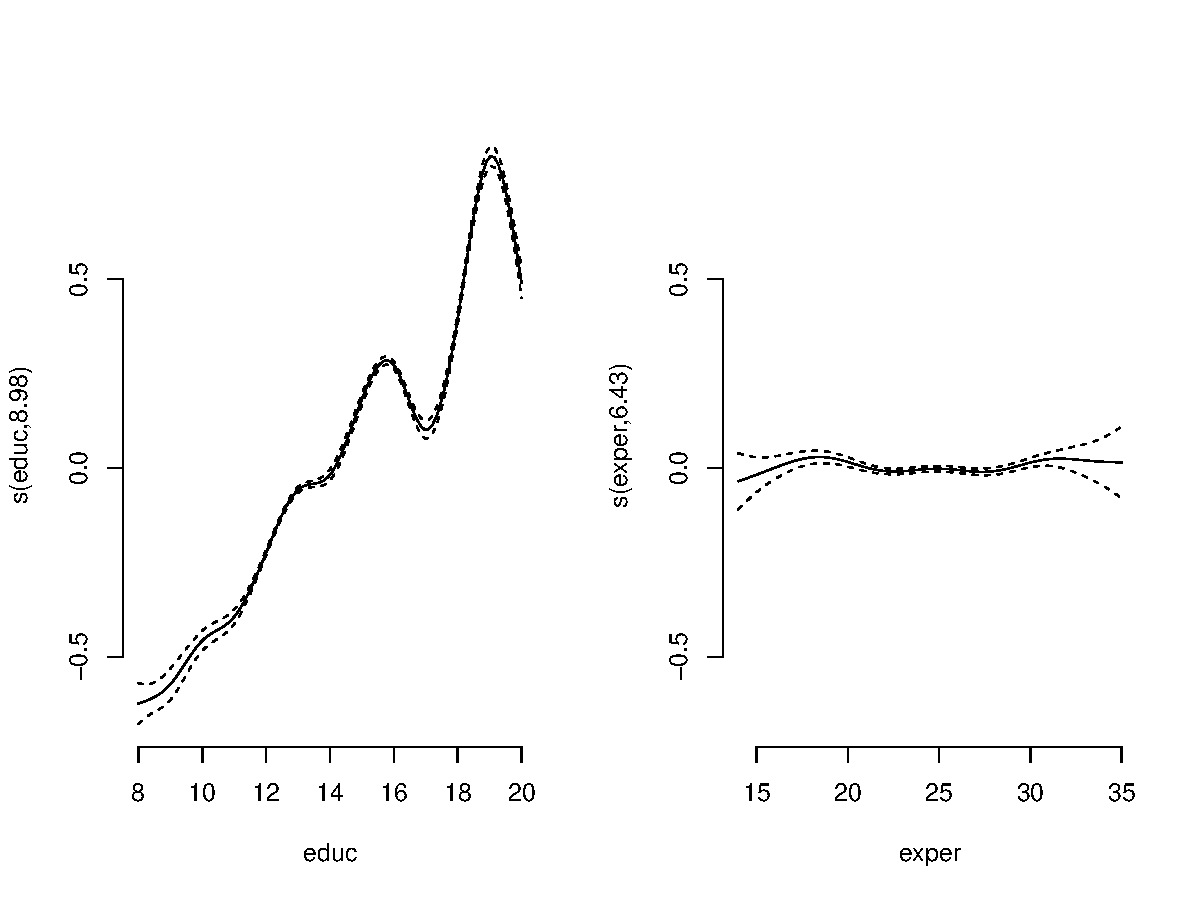
\includegraphics[width =  \textwidth]{figures/gam_wage.pdf}
\caption{Generalized additive model}\label{fig::gam-wage}
\end{figure}

The \ri{R} code in this section is in \ri{code16.2.1.R}. See \citet{wood2017generalized} for more details about the generalized additive model.



\subsection{Regression discontinuity and regression kink}


\begin{figure}
\centering 
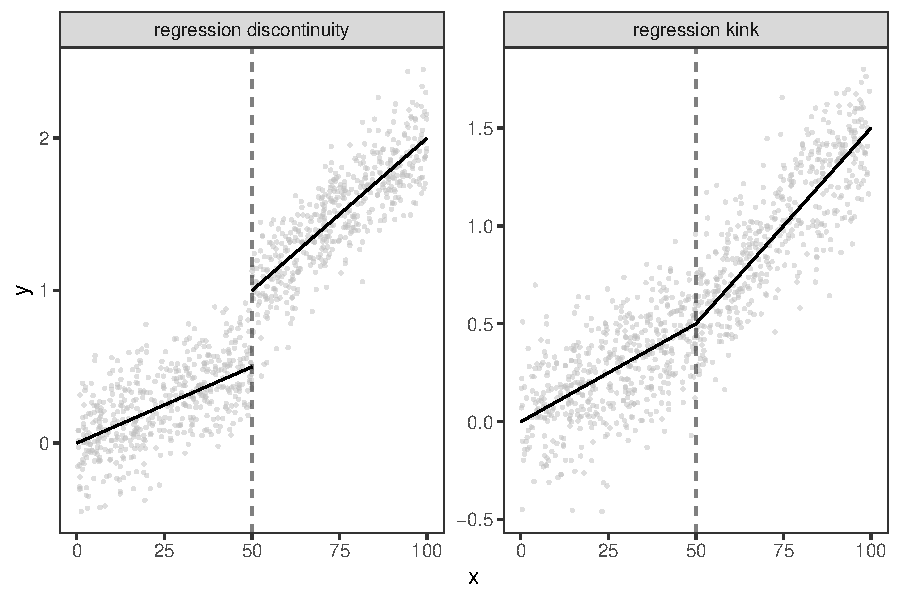
\includegraphics[width =  \textwidth]{figures/regressiondiscontinuitykink_ggplot.pdf}

\caption{Regression discontinuity and kink}\label{fig::reg-discon-kink}

\end{figure}


The left panel of Figure \ref{fig::reg-discon-kink} shows an example of regression discontinuity, where the linear functions before and after a cutoff point can differ with a possible jump. A simple way to capture the two regimes of linear regression is to fit the following model: 
\[
y_{i}=\beta_{1}+\beta_{2}x_{i}+\beta_{3}1\left(x_{i}>c\right)+\beta_{4}x_{i}1\left(x_{i}>c\right)+\varepsilon_{i}.
\]
So 
\[
y_{i}=\begin{cases}
\beta_{1}+\beta_{2}x_{i}+\varepsilon_{i} & x_{i}\leq c,\\
\left(\beta_{1}+\beta_{3}\right)+\left(\beta_{2}+\beta_{4}\right)x_{i}+\varepsilon_{i}, & x_{i}>c.
\end{cases}
\]
Testing the discontinuity at $c$ is equivalent to testing
\[
\left(\beta_{1}+\beta_{3}\right)+\left(\beta_{2}+\beta_{4}\right)c=\beta_{1}+\beta_{2}c\Longleftrightarrow\beta_{3}+\beta_{4}c=0.
\]

If we center the covariates at $c$, then 
\[
y_{i}=\beta_{1}+\beta_{2}(x_{i}-c)+\beta_{3}1\left(x_{i}>c\right)+\beta_{4}(x_{i}-c)1\left(x_{i}>c\right)+\varepsilon_{i}
\]
and
\[
y_{i}=\begin{cases}
\beta_{1}+\beta_{2}(x_{i}-c)+\varepsilon_{i} & x_{i}\leq c,\\
\left(\beta_{1}+\beta_{3}\right)+\left(\beta_{2}+\beta_{4}\right)(x_{i}-c)+\varepsilon_{i}, & x_{i}>c.
\end{cases}
\]
So testing the discontinuity at $c$ is equivalent to testing $\beta_{3}=0$. 

The right panel of Figure \ref{fig::reg-discon-kink} shows an example of regression kink, where the linear functions before and after a cutoff point can differ but the whole regression line is continuous. A simple way to capture the two regimes of linear regression is to fit the following model: 
\[
y_{i}=\beta_{1}+\beta_{2}R_{c}(x_{i})+\beta_{3}(x_{i}-c)+\varepsilon_{i}
\]
using  
\[
R_{c}(x)=\max(0,x-c)=\begin{cases}
0, & x\leq c,\\
x-c, & x>c.
\end{cases}
\]
So 
\[
y_{i}=\begin{cases}
\beta_{1}+\beta_{3}(x_{i}-c)+\varepsilon_{i}, & x_{i}\leq c,\\
\beta_{1}+\left(\beta_{2}+\beta_{3}\right)(x_{i}-c)+\varepsilon_{i}, & x_{i}>c.
\end{cases}
\]
This ensures that the mean function is continuous at $c$ with both
left and right limits equaling $\beta_{1}$. Testing the kink is equivalent
to testing $\beta_{2}=0.$


These regressions have many applications in economics, but I omit the economic background. Readers can find more discussions in  \citet{angrist2008mostly} and \citet{card2015inference}.



\section{Homework problems}


\paragraph{Piecewise linear regression}

Generate data in the same way as the example in Figure \ref{fig::npreg-basis}, and fit a continuous piecewise linear function with cutoff points $0,0.2,0.4,0.6,0.8,1$. 

 

